\chapter{Derivations and proofs}

This appendix contains derivations and proofs for some of the statements made throughout the thesis. A note on notation: In order to shorten some equations, $\cos(\alpha)$ and $\sin(\alpha)$ are replaced by the shorter $c_\alpha$ and $s_\alpha$.

\section{Probabilistic landmark model}

\subsection{Covariance matrix transformation}

\label{proof:covariance_matrix_transformation}

\begin{figure}[t]
 \begin{center}
  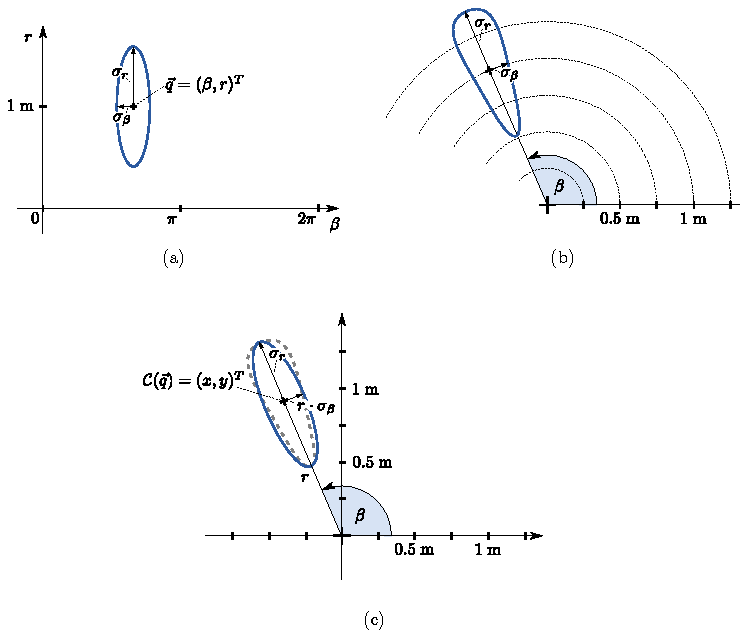
\includegraphics[width=0.975\textwidth]{media/gauss_cartesian.pdf}
 \end{center}
 \caption{Idea of the covariance matrix transformation from polar coordinates to Cartesian coordinates. (a) Shows a contour of the original Gaussian distribution in polar space. (b) Shows the same distribution drawn in a polar coordinate system. Note how the distribution is distorted. (c) Shows the approximated Gaussian distribution in a Cartesian coordinate system. The distortion present in (b) is discarded. The angular variance $\sigma_\beta$ is transformed to Cartesian coordinates by multiplication with the radius $r$. The covariance matrix of the Cartesian distribution is then calculated by rotating the Eigenraum of the original covariance matrix.}
 \label{fig:gauss_cartesian}
\end{figure}

The covariance matrix of the Gaussian distribution for polar coordinates $\vec q = (\beta, r)^T$ was given in equation \ref{eqn:gaussian_polar} as
\begin{equation*}
  \vec q_R \sim \mathcal{N}\left(\vec q_E, \Sigma(\vec q_E) \right) \text{ where } \Sigma(\beta, r) := \begmat \sigma_\beta^2 & 0 \\ 0 & \sigma_r^2 \finmat \; .
\end{equation*}
This distribution can be estimated by a Gaussian distribution in Cartesian space (see figure \ref{fig:gauss_cartesian} for an overview). Note that the estimation introduces a small bias towards smaller distances. The magnitude of this bias depends on the ratio of $\sigma_\beta$ to $\sigma_r$. The estimation is performed by choosing a covariance matrix $\Sigma_{\mathcal{C}}$ with Eigenvectors pointing in radial direction and the corresponding orthogonal direction. The Eigenvectors $\vec v_r, \vec v_\beta$ of $\Sigma_{\mathcal{C}}$ should hence have the following form:
\begin{align*}
 \vec v_r &= \begmat c_\beta \\ s_\beta \finmat & \vec v_\beta &= \begmat -s_\beta \\ c_\beta \finmat^T
\end{align*}
The Eigenvalues of a Covariance matrix correspond to the squared standard deviations of the elementary distributions:
\begin{align*}
 \lambda_r &= \sigma_r^2 &
 \lambda_\beta &= (r \cdot \sigma_\beta)^2
\end{align*}
The angular standard deviation needs to be multiplied with $r$, as in Cartesian coordinates the length of the underlying circle segment scales with the radius. The desired $\Sigma_{\mathcal{C}} = \begmat a & b \\ b & c \finmat$ can now be described by the following equations:
\begin{align*}
	 \Sigma_{\mathcal{C}} \cdot \vec v_r = \begmat a & b \\ b & c \finmat \begmat  c_\beta \\  s_\beta \finmat &= \lambda_r \begmat c_\beta \\  s_\beta \finmat \\
	 \Sigma_{\mathcal{C}} \cdot \vec v_\beta = \begmat a & b \\ b & c \finmat \begmat -s_\beta \\  c_\beta \finmat &= \lambda_\beta \begmat -s_\beta \\ c_\beta \finmat
\end{align*}
Solving the equations for $b$ yields:
\begin{align*}
	b &= \frac{(\lambda_r - a)  \cdot c_\beta}{s_\beta}
	= \frac{(\lambda_r - c)  \cdot s_\beta}{c_\beta}
	= \frac{(a - \lambda_\beta) \cdot s_ \beta}{c_\beta}
	= \frac{(c - \lambda_\beta) \cdot c_\beta}{s_\beta}
\end{align*}
Solve these equalities for $a$, $c$ and $b$:
\begin{align*}
	a &= \lambda_r c_\beta^2 + \lambda_\beta s_\beta^2 \\
	c &= \lambda_r s_\beta^2 + \lambda_\beta c_\beta^2 \\
	b &= \left(\lambda_r (1 - c_\beta^2) + \lambda_\beta s_\beta^2 \right) \frac{c_\beta}{s_\beta}
	  = \left(\lambda_r c_\beta^2 + \lambda_\beta (s_\beta^2 - 1) \right) \frac{s_\beta}{c_\beta}
	  = c_\beta s_\beta (\lambda_r - \lambda_\beta)
\end{align*}
The Cartesian approximate of the polar covariance matrix is thus given as:
\begin{align*}
	\Sigma_{\mathcal{C}}(\beta, r) &= \begmat
	    (\sigma_r c_\beta)^2 + (r \sigma_\beta s_\beta)^2 & c_\beta s_\beta (\sigma_r^2 - (r \sigma_\beta)^2) \\
	    c_\beta s_\beta (\sigma_r^2 - (r \sigma_\beta)^2) & (\sigma_r s_\beta)^2 + (r \sigma_\beta c_\beta)^2
	\finmat
\end{align*}


\subsection{Derivation of $\sigma_\beta$ for adjacent Gaussian distributions}

\label{proof:sigma_beta}

The angular variance $\sigma_\beta$ used in equation \ref{eqn:sigma_beta} is derived by demanding that the sum two adjacent Gaussian distributions ($\mu_1 = \mu_2 + \Delta \beta$) nearly forms a uniform distribution in the interval $[\mu_1, \mu_2]$ as shown in figure \ref{fig:sigma_beta}. The variance can be derived as a solution to the following more general problem:

Given the sum of two (one dimensional) Gaussian distributions with means $\mu_1$ and $\mu_2$ (where $\zeta := \mu_2 - \mu_1$) and a common variance $\sigma$:
  $$f(x) = \mathcal{N}(x \mid \mu_1, \sigma) + \mathcal{N}(x \mid \mu_2, \sigma)$$
Goal: Find $\sigma$ such that second derivative of $f(x)$ at $x = \mu_1 + \nicefrac{\zeta}2$ equals zero:
  $$\left. \frac{\partial f}{\partial x^2} \right|_{x = \mu_1 + \nicefrac{\zeta}2} \overset{!}= 0$$
By shifting $\mu_1 + \nicefrac{\zeta}2$ to the origin, the equation can be rewritten as:
  $$
  \left. \frac{\partial f\left(x - \mu_1 - \nicefrac{\zeta}2\right)}{\partial x^2} \right|_{x = 0} = \left. \frac{\partial}{\partial x^2} \; \left( \mathcal{N}\left(x \mid -\nicefrac{\zeta}2, \sigma\right) + \mathcal{N}\left(x \mid \nicefrac{\zeta}2, \sigma\right) \right) \right|_{x = 0} \overset{!}= 0$$
Derivation and evaluation at $x = 0$ yield ($\alpha$ represents all omitted normalization and constant factors):
  $$\left. \frac{\partial}{\partial x^2} \; \left( \mathcal{N}\left(x \mid -\nicefrac{\zeta}2, \sigma\right) + \mathcal{N}\left(x \mid \nicefrac{\zeta}2, \sigma\right) \right) \right|_{x = 0} = \alpha \cdot \frac{\exp\left(-\frac{\zeta^2}{8 \, \sigma^2}\right)}{\sigma^5} \left( -4\,\sigma^2+\zeta^2 \right) \overset{!}= 0$$
The solution for $\sigma$ is then given as
  $$\sigma = \pm \frac{\zeta}2 \; .$$
Setting $\zeta = \Delta \beta$ yields the term used in equation \ref{eqn:sigma_beta}.

\section{Motion field equation}

\subsection{Substitution of $r$ and $d$}

\label{proof:flow_subst}

The parameters $r$ and $d$ of equation \ref{eqn:motion_field_vector} are redundant and can be substituted by a single parameter $\rho := \frac{d}{r}$.

\begin{proof}
Equation \ref{eqn:motion_field_vector} was given as
\begin{align*}
\vec u(\vec p; T(d, \psi, \alpha), r) &= \begmat
  \beta' - \beta \\
  \gamma' - \gamma
\finmat \; .
\end{align*}
Expand the equation as defined in \ref{eqn:project}, \ref{eqn:unproject} and \ref{eqn:transform}. As $\atantwo(y, x)$ only selects the sign of the result depending on the quadrant of the input vector, $\atantwo(y, x)$ is substituted by $\arctan(\nicefrac{y}x)$ in this proof.
\begin{align*}
\beta' &= \arctan
    \left(
      \frac{
	- r s_{\psi} c_\beta + r c_{\psi} s_\beta + d s_{\alpha}
      }{
          r c_{\psi} c_\beta + r s_{\psi} s_\beta + d c_{\alpha}
      }
    \right) \\
    &= \arctan
    \left(
      \frac{
	  r \cdot (-s_{\psi} c_\beta + c_{\psi} s_\beta + \rho s_{\alpha} )
      }{
          r \cdot ( c_{\psi} c_\beta + s_{\psi} s_\beta + \rho c_{\alpha} )
      }
    \right) \\
    &= \arctan
    \left(
      \frac{
	  -s_{\psi} c_\beta + c_{\psi} s_\beta + \rho s_{\alpha}
      }{
          c_{\psi} c_\beta + s_{\psi} s_\beta + \rho c_{\alpha}
      }
    \right) \\
\gamma' &= \arctan
    \left(
      \frac{
	r \cdot \tan(\gamma)
      }{
	\sqrt{
	  (  r c_{\psi} c_\beta + r s_{\psi} s_\beta + d c_{\alpha})^{2} +
	  (- r s_{\psi} c_\beta + r c_{\psi} s_\beta + d s_{\alpha})^{2}}
      }
    \right) \\
    &= \arctan
    \left(
      \frac{
	r \cdot \tan(\gamma)
      }{
	r \cdot \sqrt{
	  (  c_{\psi} c_\beta + s_{\psi} s_\beta + \rho c_{\alpha})^{2} +
	  (- s_{\psi} c_\beta + c_{\psi} s_\beta + \rho s_{\alpha})^{2}}
      }
    \right)\\
    &= \arctan
    \left(
      \frac{
	\tan(\gamma)
      }{
	\sqrt{
	  (  c_{\psi} c_\beta + s_{\psi} s_\beta + \rho c_{\alpha})^{2} +
	  (- s_{\psi} c_\beta + c_{\psi} s_\beta + \rho s_{\alpha})^{2}}
      }
    \right)
\end{align*}
\end{proof}

\subsection{Rotational motion elimination}

\label{proof:rot_motion_elim}

It was stated in equation \ref{eqn:rot_motion_elim}:
  $$\vec u(\vec p; \psi, \alpha, \rho) = \vec u(\vec p - (\psi + \alpha, 0)^T; 0, 0, \rho) - (\psi, 0)^T$$

\begin{proof}
Prove the equation in two steps using the results derived in the previous section \ref{proof:flow_subst}:
\begin{enumerate}[1.]
 \item It holds $\vec u(\vec p; \alpha, \psi, \rho) = \vec u(\vec p - (\psi, 0)^T; \alpha, 0, \rho) - (\psi, 0)^T$. Apply the addition theorems:
 \begin{align*}
\beta'(\beta, \psi) &= \arctan
    \left(
      \frac{
	  -s_{\psi} c_\beta + c_{\psi} s_\beta + \rho s_{\alpha}
      }{
          c_{\psi} c_\beta + s_{\psi} s_\beta + \rho c_{\alpha}
      }
    \right) & \\
    &= \arctan\left(
      \frac{
	  \sin(\beta - \psi) + \rho s_{\alpha}
      }{
          \cos(\beta - \psi) + \rho c_{\alpha}
      }
    \right) \\
    &= \beta'(\beta - \psi, 0) \\
\gamma'(\beta, \psi) &= \arctan
    \left(
      \frac{
	\tan(\gamma)
      }{
	\sqrt{
	  (  c_{\psi} c_\beta + s_{\psi} s_\beta + \rho c_{\alpha})^{2} +
	  (- s_{\psi} c_\beta + c_{\psi} s_\beta + \rho s_{\alpha})^{2}}
      }
    \right) \\
    &= \arctan
    \left(
      \frac{
	r \cdot \tan(\gamma)
      }{
	r \cdot \sqrt{
	  (  \cos(\beta - \psi) + \rho c_{\alpha} )^{2} +
	  (  \sin(\beta - \psi) + \rho s_{\alpha})^{2}}
      }
    \right)\\
    &= \gamma'(\beta - \psi, 0)
\end{align*}
Plug these results into the definition of $\vec u$:
\begin{align}
\begin{aligned}
  \vec u(\vec p; \psi, \alpha, \rho) &=
  \begmat
    \beta'(\beta, \psi) - \beta \\
    \gamma'(\beta, \psi) - \gamma
  \finmat \\
  &= \begmat
    \beta'(\beta - \psi, 0) - \beta + \psi \\
    \gamma'(\beta - \psi, 0) - \gamma \\
  \finmat \\
  &= \vec u(\vec p - (\psi, 0)^T; \alpha, 0, \rho) - (\psi, 0)^T
\end{aligned}
\label{eqn:flow_prf1}
\end{align}
  \item It holds $\vec u(\vec p; \alpha, 0, \rho) = \vec u(\vec p - (\alpha, 0)^T; 0, 0, \rho)$. Expand the argument of the arctangent in $\beta'(\beta + \alpha, \alpha)$ using the addition theorems and reorder:
\begin{align*}
 \beta'(\beta - \alpha, \alpha) &{\overset{\phantom{\text{Rot. Mat.}\;}}=} \arctan
    \left(
      \frac{
	  \sin(\beta - \alpha) + \rho s_{\alpha}
      }{
          \cos(\beta - \alpha) + \rho c_{\alpha}
      }
    \right) \\
    &{\overset{\phantom{\text{Rot. Mat.}\;}}=} \arctan
    \left(
      \frac{
	  c_\alpha s_\beta - s_\alpha (c_\beta + \rho)
      }{
	  s_\alpha s_\beta + c_\alpha (c_\beta + \rho)
      }
    \right) \\
    &{\overset{\text{Rot. Mat.}\;}=} \arctan
    \left(
      \frac{
	  s_\beta
      }{
	  c_\beta + \rho
      }
    \right) + \alpha \\
    &{\overset{\phantom{\text{Rot. Mat.}\;}}=} \beta'(\beta, 0) - \alpha
\end{align*}
Analogously it holds for $\gamma'(\beta - \alpha, \alpha)$:
\begin{align*}
  \gamma'(\beta - \alpha, \alpha) &= \arctan
    \left(
      \frac{
	r \cdot \tan(\gamma)
      }{
	r \cdot \sqrt{
	  (  \cos(\beta - \alpha) + \rho c_{\alpha} )^{2} +
	  (  \sin(\beta - \alpha) + \rho s_{\alpha})^{2}}
      }
    \right) \\
    &= \arctan
    \left(
      \frac{
	r \cdot \tan(\gamma)
      }{
	r \cdot \sqrt{
	  (  s_\alpha s_\beta + c_\alpha (c_\beta + \rho) )^{2} +
	  (  c_\alpha s_\beta - s_\alpha (c_\beta + \rho) )^{2}}
      }
    \right) \\
    &= \arctan
    \left(
      \frac{
	r \cdot \tan(\gamma)
      }{
	r \cdot \sqrt{
	  (  c_\beta + \rho )^{2} +
	  (  s_\beta )^{2}}
      }
    \right) \\
    &= \gamma'(\beta, 0)
\end{align*}
Plug these results into the definition of $\vec u$:
\begin{align}
\begin{aligned}
\vec u(\vec p - (\alpha, 0)^T; 0, 0, \rho) &= \begmat
    \beta'(\beta - \alpha, \alpha) - \beta + \alpha \\
    \gamma'(\beta - \alpha, \alpha)
  \finmat \\
  &= \begmat
    \beta'(\beta, 0) - \beta \\
    \gamma'(\beta, 0)
  \finmat \\
  &= \vec u(\vec p; \alpha, 0, \rho)
\end{aligned}
\label{eqn:flow_prf2}
\end{align}
\end{enumerate}
Combining the results from equations \ref{eqn:flow_prf1} and \ref{eqn:flow_prf2} yields the desired equation.
\end{proof}

\subsection{Maximum horizontal shift}

\label{proof:max_horz_shift}

\begin{figure}[htb]
\begin{center}
 \subbottom[\label{fig:max_horz_shift}]{
 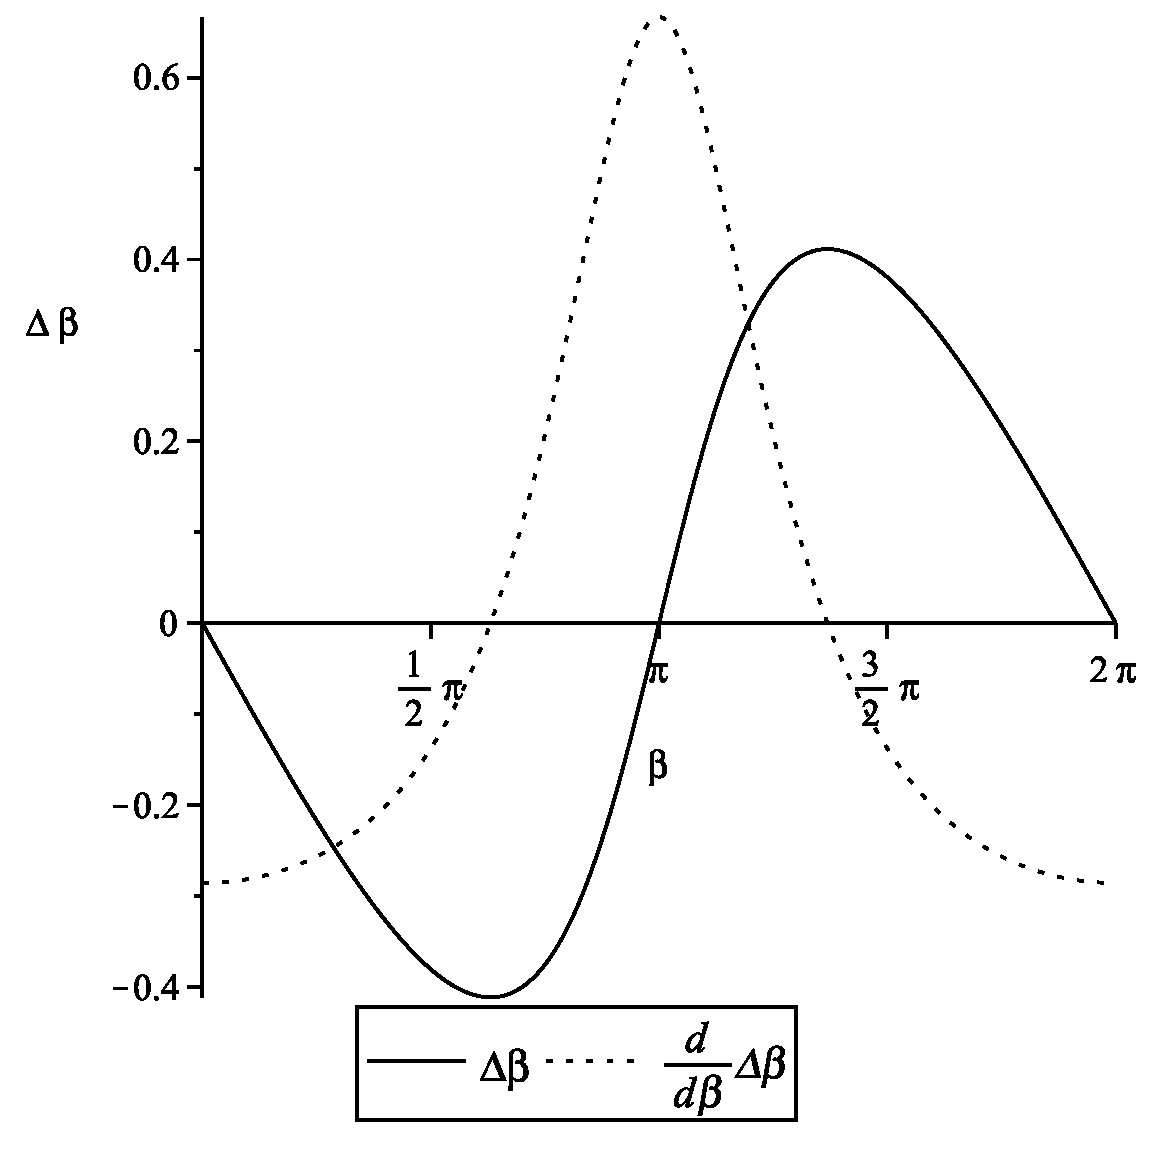
\includegraphics[width=0.475\textwidth]{media/max_horz_shift.pdf}}
 \subbottom[\label{fig:horz_shift_comparison}]{
 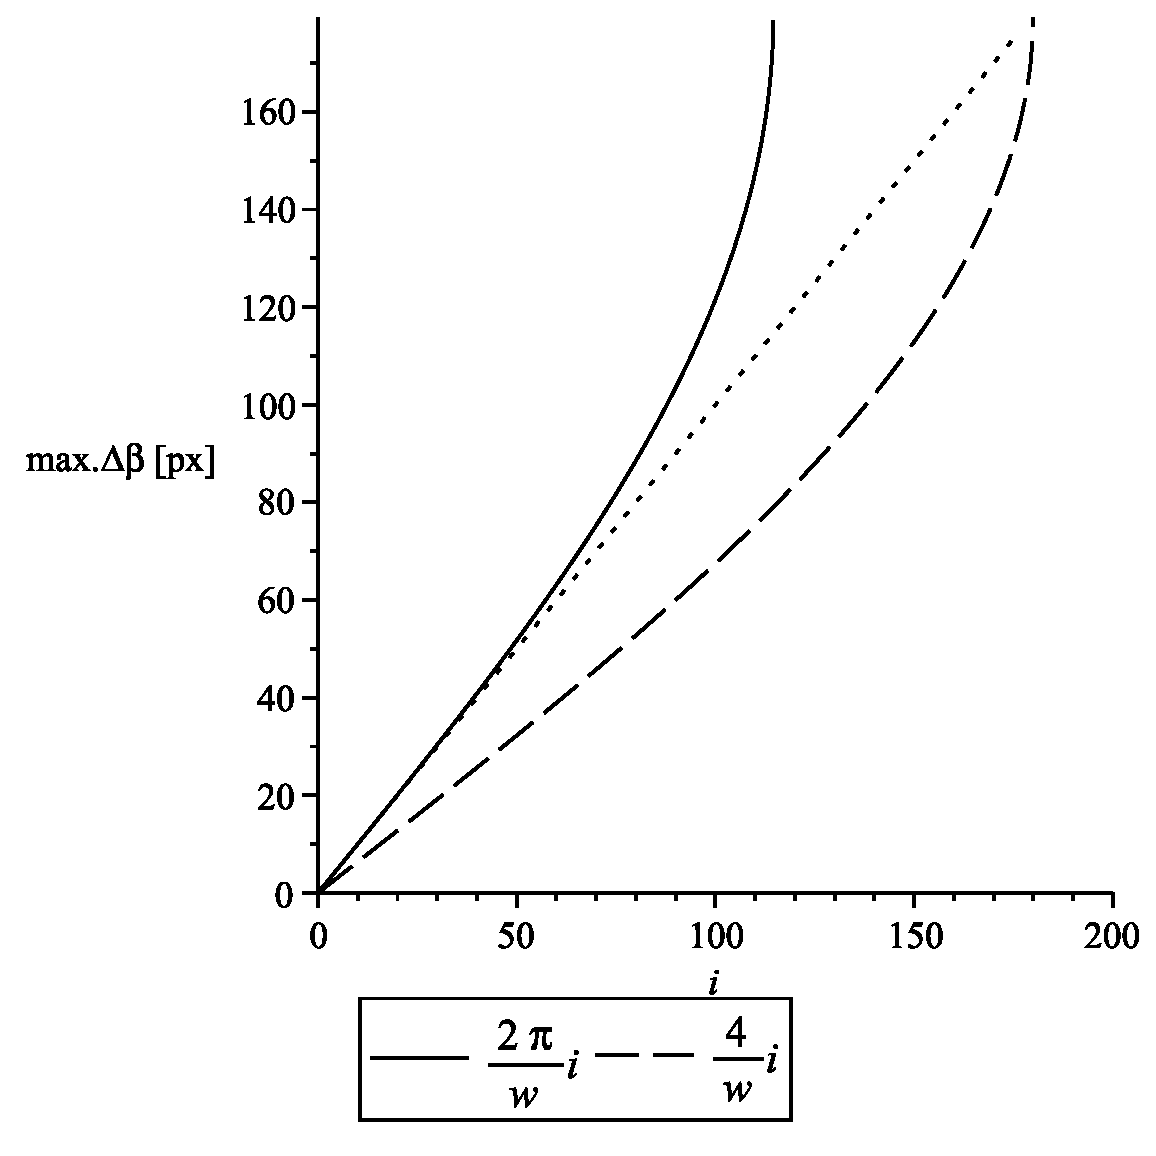
\includegraphics[width=0.475\textwidth]{media/horz_shift_comparison.pdf}}
\end{center}
\caption{(a) Plot of $\Delta \beta(\beta)$ and its derivative for $\rho = 0.4$. (b) A plot of the horizontal shift in pixels at $\hat \beta$ for both approximations presented below. The image width was set to $w = 720$. The dotted line represents the aimed-at behavior as achieved by the analytical solution.}
\end{figure}

In section \ref{sec:index_to_depth} the formula $\rho_i = \frac{2\pi}{w} \cdot i$ was introduced, which approximately ensures the horizontal motion field shift $\Delta \beta(\beta) = \beta'(\beta) - \beta$ to be smaller than one pixel per step for $0 \leq \rho \ll 1$.

\begin{derivation}
The shift in horizontal direction $\Delta \beta(\beta)$ is given as:
  $$\Delta \beta(\beta) = \beta'(\beta) - \beta = \atantwo \left(\sin(\beta), \cos(\beta) + \rho \right) - \beta$$
The extrema of this function can be found by calculating the first derivative and equating it with zero:
\begin{align*}
   \frac{\mathrm{d}}{\mathrm{d} \beta} \, \Delta \beta(\beta)&= \frac{\mathrm{d}}{\mathrm{d}\beta} \left( \atantwo \left(\sin(\beta), \cos(\beta) + \rho\right) - \beta \right)\\
     &= \frac{\cos(\beta)^2 + \rho \cos(\beta) + \sin(\beta)^2}{(\cos(\beta) + \rho)^2} \cdot
       \frac{(\cos(\beta) + \rho)^2}{(\cos(\beta) + \rho)^2 + \sin(\beta)^2} - 1\\
     &= \frac{(\cos(\beta) + \rho)^2 + \sin(\beta)^2 - \cos(\beta) \rho - \rho^2}{(\cos(\beta) + \rho)^2 + \sin(\beta)^2} - 1\\
     &= - \frac{\rho \cdot (\cos(\beta) + \rho)}{(\cos(\beta) + \rho)^2 + \sin(\beta)^2}
     \overset{!}= 0 \\
  \Leftrightarrow 0 &= \cos(\beta) + \rho \\
  \Leftrightarrow \beta &= \underbrace{\pm\arccos(-\rho)}_{=: \hat \beta}
\end{align*}
Note that this solution is only valid for $0 \leq \rho \leq 1$. Plugging this result into $\Delta \beta$ and equating $\Delta \beta(\hat \beta)$ for multiples of the horizontal image resolution $\frac{2\pi}{w}$ (with $w$ being the image width in pixels) results in the following equation:
\begin{align*}
  \Delta \beta(\hat \beta) &= \atantwo \left(\sin(\pm\arccos(-\rho_i)), \cos(\arccos(-\rho_i)) + \rho_i \right) \mp \arccos(-\rho_i)\displaybreak[3]\\
  &= \atantwo \left(\pm\sqrt{1 - \rho_i^2}, 0 \right) \mp \arccos(-\rho_i)\displaybreak[3]\\
  &= \pm \frac{\pi}2 \mp \arccos(-\rho_i)
  \overset{!}\leq \frac{2\pi}{w} \cdot i
\end{align*}
An analytical solution that ensures equality is achieved for
$$\rho_i = - \cos\left(\frac{2\pi}w \cdot i + \frac{\pi}2\right) = \sin\left(\frac{2\pi}w \cdot i \right) \; .$$
For small $\frac{2\pi}w \cdot i$ the analytical solution can be approximated as:
\begin{equation*}
  \rho_i \approx \frac{2\pi}{w} \cdot i
\end{equation*}
As can be seen in figure \ref{fig:horz_shift_comparison} the approximation seems to be acceptable for $i < 40$ and $w = 720\;\mathrm{px}$. In the current implementation only $32$ error stack layers ($0 \leq i \leq 31$) are used.

A solution which ensures that the inequality stated above is always fulfilled can be obtained by linearly estimating the arctangent. It holds:
  $$-\frac{\pi}2 + \arccos(-\rho_i) \leq \frac{\pi}2 \cdot \rho_i \overset{!}\leq \frac{2\pi}{w} \cdot i \; .$$
Solving the right part of the inequality for $\rho_i$ results in
\begin{equation*}
  \rho_i \leq \frac{4}{w} \cdot i
\end{equation*}
which allows to fulfill the requirement for all $0 \leq \rho_i \leq 1$ (see figure \ref{fig:horz_shift_comparison} for a comparison to the approximation).
\end{derivation}
